\documentclass[a4paper]{arrowhead}

\usepackage[yyyymmdd]{datetime}
\usepackage{etoolbox}
\usepackage[utf8]{inputenc}
\usepackage{multirow}

\renewcommand{\dateseparator}{-}

\setlength{\parskip}{1em}

%% Special references
\newcommand{\fref}[1]{{\textcolor{ArrowheadBlue}{\hyperref[sec:functions:#1]{#1}}}}
\newcommand{\mref}[1]{{\textcolor{ArrowheadPurple}{\hyperref[sec:model:#1]{#1}}}}
\newcommand{\pdef}[1]{{\textcolor{ArrowheadGrey}{#1\label{sec:model:primitives:#1}\label{sec:model:primitives:#1s}\label{sec:model:primitives:#1es}}}}
\newcommand{\pref}[1]{{\textcolor{ArrowheadGrey}{\hyperref[sec:model:primitives:#1]{#1}}}}

\newrobustcmd\fsubsection[3]{
  \addtocounter{subsection}{1}
  \addcontentsline{toc}{subsection}{\protect\numberline{\thesubsection}interface \textcolor{ArrowheadBlue}{#1}}
  \renewcommand*{\do}[1]{\rref{##1},\ }
  \subsection*{
    \thesubsection\quad
    interface
    \textcolor{ArrowheadBlue}{#1}
    (\notblank{#2}{\mref{#2}}{})
    \notblank{#3}{: \mref{#3}}{}
  }
  \label{sec:functions:#1}
}
\newrobustcmd\msubsection[2]{
  \addtocounter{subsection}{1}
  \addcontentsline{toc}{subsection}{\protect\numberline{\thesubsection}#1 \textcolor{ArrowheadPurple}{#2}}
  \subsection*{\thesubsection\quad#1 \textcolor{ArrowheadPurple}{#2}}
  \label{sec:model:#2} \label{sec:model:#2s} \label{sec:model:#2es}
}
\newrobustcmd\msubsubsection[3]{
  \addtocounter{subsubsection}{1}
  \addcontentsline{toc}{subsubsection}{\protect\numberline{\thesubsubsection}#1 \textcolor{ArrowheadPurple}{#2}}
  \subsubsection*{\thesubsubsection\quad#1 \textcolor{ArrowheadPurple}{#2}}
  \label{sec:model:#2} \label{sec:model:#2s}
}
%%

\begin{document}

%% Arrowhead Document Properties
\ArrowheadTitle{orchestration-service} % XXX = ServiceName 
\ArrowheadServiceID{orchestration-service} % ID name of service
\ArrowheadType{Service Description}
\ArrowheadTypeShort{SD}
\ArrowheadVersion{4.6.0} % Arrowhead version X.Y.Z, e..g. 4.4.1
\ArrowheadDate{\today}
\ArrowheadAuthor{Rajmund Bocsi} % Corresponding author e.g. Jerker Delsing
\ArrowheadStatus{RELEASE} % e..g. RELEASE, RELEASE CONDIDATE, PROTOTYPE
\ArrowheadContact{rbocsi@aitia.ai} % Email of corresponding author
\ArrowheadFooter{\href{www.arrowhead.eu}{www.arrowhead.eu}}
\ArrowheadSetup
%%

%% Front Page
\begin{center}
  \vspace*{1cm}
  \huge{\arrowtitle}

  \vspace*{0.2cm}
  \LARGE{\arrowtype}
  \vspace*{1cm}

  %\Large{Service ID: \textit{"\arrowid"}}
  \vspace*{\fill}

  % Front Page Image
  %\includegraphics{figures/TODO}

  \vspace*{1cm}
  \vspace*{\fill}

  % Front Page Abstract
  \begin{abstract}
    This document provides service description for the \textbf{orchestration-service} service. 
  \end{abstract}

  \vspace*{1cm}

%   \scriptsize
%   \begin{tabularx}{\textwidth}{l X}
%     \raisebox{-0.5\height}{
\includegraphics[width=2cm]{figures/artemis_logo}} & {ARTEMIS Innovation Pilot Project: Arrowhead\newline
%     THEME [SP1-JTI-ARTEMIS-2012-AIPP4 SP1-JTI-ARTEMIS-2012-AIPP6]\newline
%     [Production and Energy System Automation Intelligent-Built environment and urban infrastructure for sustainable and friendly cities]}
%   \end{tabularx}
%   \vspace*{-0.2cm}
 \end{center}

\newpage
%%

%% Table of Contents
\tableofcontents
\newpage
%%

\section{Overview}
\label{sec:overview}
This document describes the \textbf{orchestration-service} service that provides runtime (late) binding between application systems. Its primary purpose is to provide application systems with orchestration information: where they need to connect to. The outcome of the service includes data that will tell the application system what service provider system(s) it should connect to and how (acting as a service consumer). Such orchestration data include:

\begin{itemize}
    \item Accessibility information details of a service provider (e.g network address and port),
    \item Details of the service instance within the provider system (e.g. base URL, IDD specification and other metadata),
    \item Authorization-related information (e.g. access token and signature),
    \item Additional information that is necessary for establishing connection.
\end{itemize}

The rest of this document is organized as follows.
In Section \ref{sec:functions}, we describe the abstract message functions provided by the service.
In Section \ref{sec:model}, we end the document by presenting the data types used by the mentioned functions.

\subsection{How This Service Is Meant to Be Used}
The given system should consume the Service Registry Core System's \textbf{query} service to get information about the \textbf{orchestration-service} service. Using this information the system can request the \textbf{orchestration-service} service with an orchestration form about the service the system wants to consume. 

The service can be used in two ways. The first one uses predefined rules (coming from the fix or flexible database store) to find the appropriate providers for the consumer. The second option is the dynamic orchestration in which case the service searches the whole local cloud (and maybe some other clouds) to find matching providers.

\subsubsection{Fix Store Orchestration}

\begin{itemize}
    \item requester system is mandatory,
    \item requested service and all the other parameters are optional,
    \item if requested service is not specified, then this service returns the top priority local provider of all services contained by the Orchestrator store database for the requester system. if requested service is specified, then it has to contain the service definition and exactly one interface (all other service requirements are optional). In this case, the process returns all accessible providers from the Orchestrator store database that provides the specified service via the specified interface to the specified consumer.
\end{itemize}

\subsubsection{Flexible Store Orchestration}

\begin{itemize}
    \item requester system is mandatory,
    \item requested service is mandatory, but just the service definition part, all other parameters of the requested service are optional,
    \item all other parameters are optional
\end{itemize}    

\subsubsection{Dynamic Orchestration}

\begin{itemize}
    \item requester system is mandatory,
    \item requested service is mandatory, but just the service definition part, all other parameters of the requested service are optional,
    \item all other parameters are optional
\end{itemize}    
    
\subsubsection{Orchestration flags}

The requester can modify the \textbf{orchestration-service}'s behaviour using these flags. These are the available options:

\begin{itemize}
    \item \texttt{enableInterCloud}: the service can search in another clouds for providers if none of the local cloud providers match the requirements,
    \item \texttt{enableQoS}: the orchestration process will use Quality-of-Service requirements and provider reservation requests (if the Orchestrator supports it),
    \item \texttt{externalServiceRequest}: the service is called by the Gatekeeper Core System on behalf of a consumer from an other cloud,
    \item \texttt{matchmaking}: the service automatically selects exactly one provider from the appropriate providers (if any),
    \item \texttt{metadataSearch}: query in the Service Registry uses metadata filtering,
    \item \texttt{onlyIPAddressResponse}: the service only returns providers whose address is an IP address (not a domain name),
    \item \texttt{onlyIPv4AddressResponse}: the service only returns providers whose address is a version 4 IP address (not a domain name and not a version 6 IP address),
    \item \texttt{onlyIPv6AddressResponse}: the service only returns providers whose address is a version 6 IP address (not a domain name and not a version 4 IP address),
    \item \texttt{onlyPreferred}: the service filters the results with the specified provider list,
    \item \texttt{overrideStore}: services uses dynamic orchestration if this flag is true, otherwise it uses the orchestration store,
    \item \texttt{pingProviders}: the service checks whether the returning providers are online and remove the in\-accessible ones from the results,
    \item \texttt{triggerInterCloud}: the service skipped the search in the local cloud and tries to find providers in other clouds instead.
\end{itemize}

\subsubsection{Quality-of-Service requirements}

If the Orchestrator Core System supports it, the requester can specify Quality-of-Service requirements when sends an orchestration request. It has to set the \texttt{enableQoS} flag to true and also provide a \texttt{qosRequirements} map. The possible keys of the map are the following:

\begin{itemize}
    \item \texttt{qosAvgRespTime}: the maximum acceptable value of the average (mean) response time, in milliseconds,
    \item \texttt{qosJitterThreshold}: the maximum acceptable value of jitter, in milliseconds,
    \item \texttt{qosMaxPacketLost}: the maximum acceptable packet loss, in percent,
    \item \texttt{qosMaxRecentPacketLoss}: the maximum acceptable recent packet loss, in percent,
    \item \texttt{qosMaxRespTimeThreshold}: the maximum acceptable value of the response time, in milliseconds,
\end{itemize}

The requester can also specify commands for the Orchestrator Core System. Currently, only one command is supported (and only if both the system and the requester enables QoS): \texttt{qosExclusivity}. With this command the requester can ask exclusive access for a provider's service for a specified time (in seconds). Exclusive access only means that the Orchestrator Core System will not include this particular provider to any orchestration result until the exclusivity expires.

\clearpage

\subsubsection{The orchestration process}

Figure \ref{fig:activity_uml} describes the orchestration process.

\begin{figure}[h!]
  \centering
  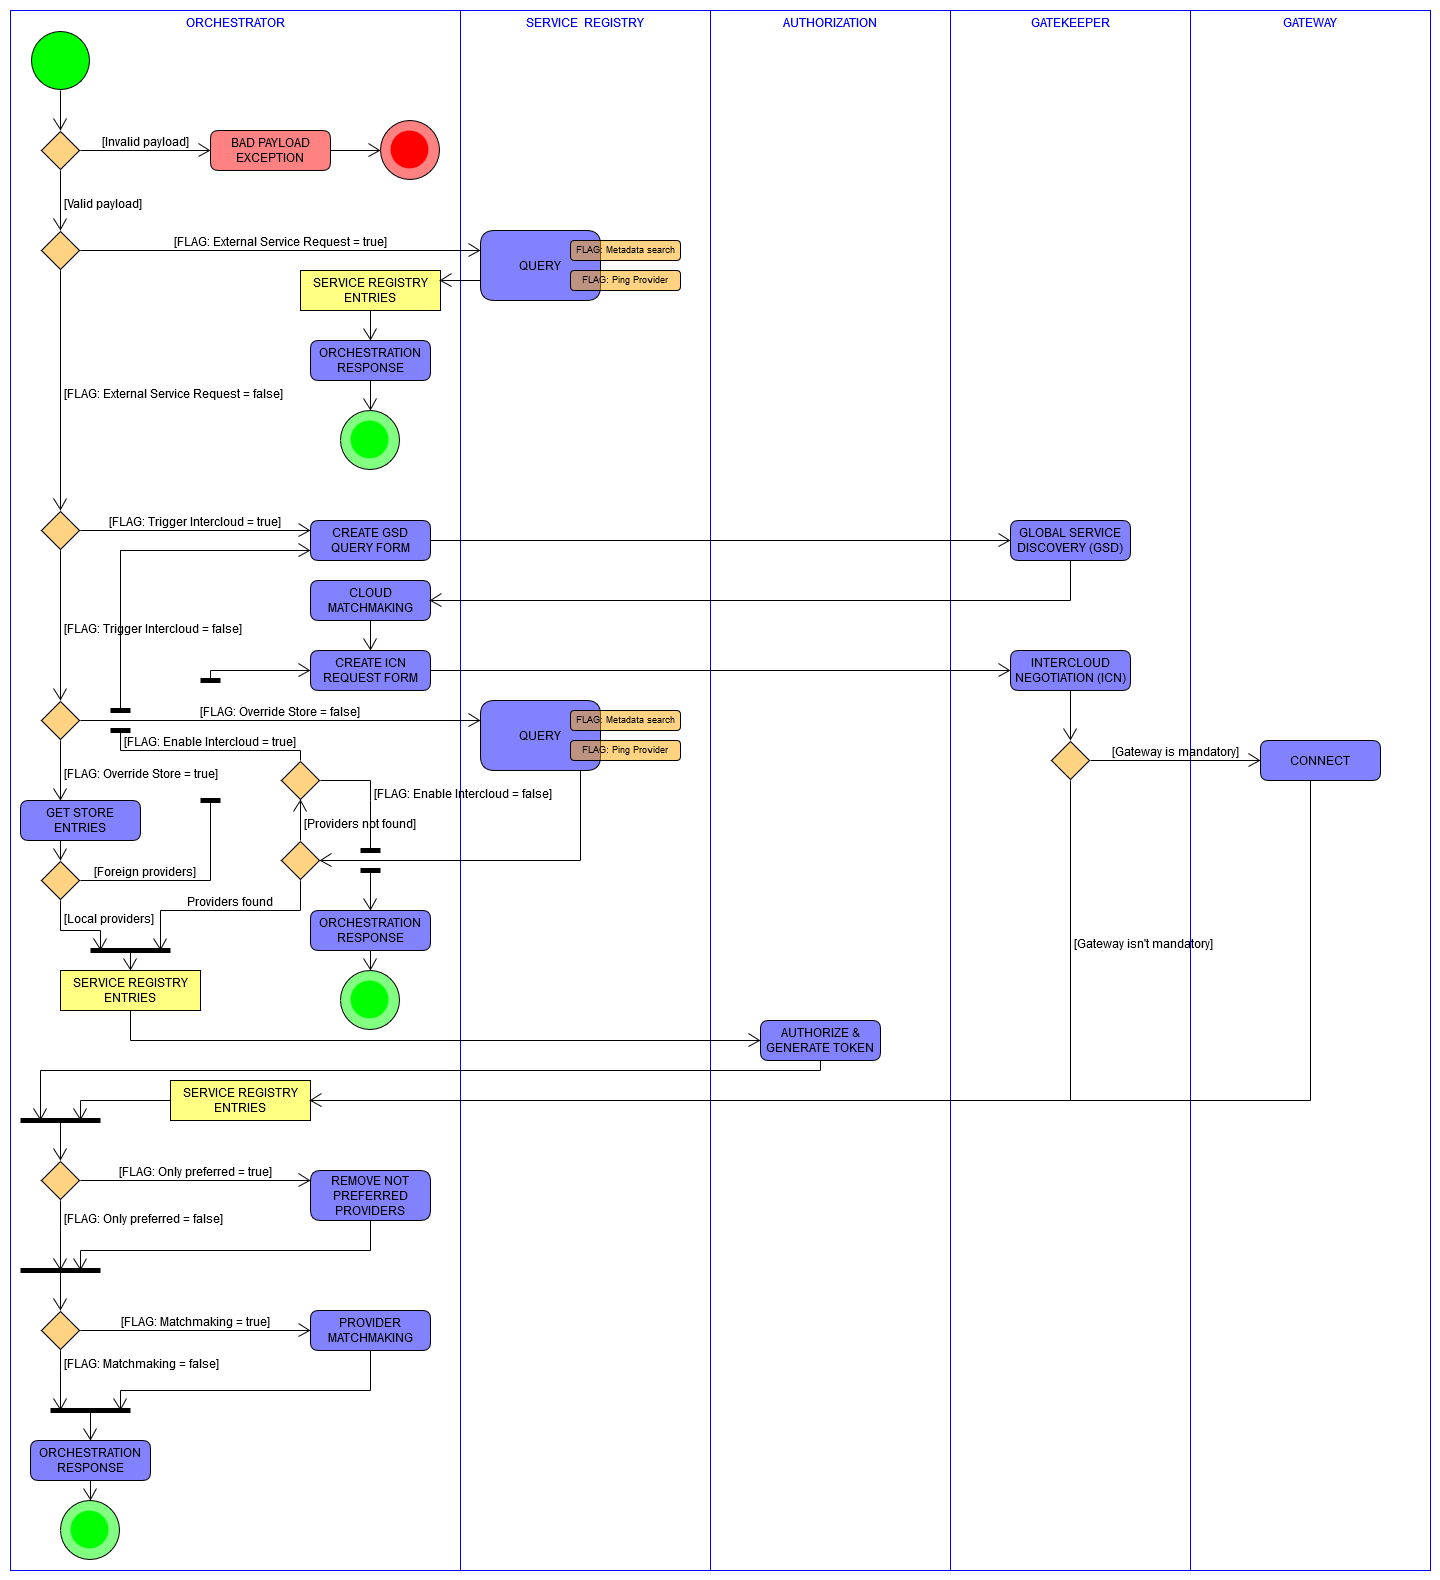
\includegraphics[width=16cm]
  {figures/post_orchestration_activity_uml}
  \caption{
    UML activity diagram of the orchestration process.
  }
  \label{fig:activity_uml}
\end{figure}

\clearpage

\subsection{Important Delimitations}
\label{sec:delimitations}

The flexible store mode has the following delimitations:

\begin{itemize}
    \item It does not support inter-cloud rules.
    \item It does not support Quality-of-Service requirements.
    \item It does not support provider reservation.
    \item It does not use the Authorization Core System to check whether a system can consume a service. Authorization should be checked before a flexible rule is inserting into the Orchestration store.
\end{itemize}

The requested service data must meet the following criteria:

\begin{itemize}
    \item Service definition can contain maximum 63 character of letters (english alphabet), numbers and dash (-), and has to start with a letter (also cannot ends with dash).
    \item Interface names have to follow the \texttt{Protocol-SecurityType-MimeType} format.
    \item Security types could be only \texttt{NOT\_SECURE}, \texttt{CERTIFICATE} or \texttt{TOKEN} .
\end{itemize}

\subsection{Access policy}
\label{sec:accesspolicy}

Available for anyone within the local cloud, but in case of application systems, the system is allowed to orchestrate only for itself. 

\newpage

\section{Service Interface}
\label{sec:functions}

This section describes the interfaces to the service. The \textbf{orchestration-service} service is used to looking for matching providers. The various parameters are representing the necessary system and service input information.
In particular, each subsection names an interface, an input type and an output type, in that order.
The input type is named inside parentheses, while the output type is preceded by a colon.
Input and output types are only denoted when accepted or returned, respectively, by the interface in question. All abstract data types named in this section are defined in Section 3.

The following interfaces are available.

\fsubsection{HTTP/TLS/JSON}{OrchestrationForm}{OrchestrationResultList}

\begin{table}[ht!]
  \centering
  \begin{tabular}{|l|l|l|l|}
    \rowcolor{gray!33} Profile type & Type & Version \\ \hline
    Transfer protocol & HTTP & 1.1 \\ \hline
    Data encryption & TLS & 1.3 \\ \hline
    Encoding & JSON & RFC 8259 \cite{rfc8259} \\ \hline
    Compression & N/A & - \\ \hline
  \end{tabular}
  \caption{HTTP/TLS/JSON communication details.}
  \label{tab:comunication_semantics_profile}
\end{table}

\clearpage

\section{Information Model}
\label{sec:model}

Here, all data objects that can be part of the \textbf{orchestration-service} service
provides to the hosting System are listed in alphabetic order.
Note that each subsection, which describes one type of object, begins with the \textit{struct} keyword, which is used to denote a collection of named fields, each with its own data type.
As a complement to the explicitly defined types in this section, there is also a list of implicit primitive types in Section \ref{sec:model:primitives}, which are used to represent things like hashes and identifiers.

\msubsection{struct}{OrchestrationForm}
\label{sec:model:OrchestrationForm}

\begin{table}[ht!]
\begin{tabularx}{\textwidth}{| p{4cm} | p{4cm} | p{2cm} | X |} \hline
\rowcolor{gray!33} Field & Type & Mandatory & Description \\ \hline
commands &\hyperref[sec:model:Metadata]{Metadata} & no & Additional commands to the Orchestrator, the only available command now is \texttt{qosExclusivity} (see above). \\ \hline
orchestrationFlags &\hyperref[sec:model:OrchestrationFlags]{OrchestrationFlags} & no & A map of flags that changes the behaviour of the service. See details above. \\ \hline
preferredProviders &\pref{List}$<$\hyperref[sec:model:PreferredProvider]{PreferredProvider}$>$ & no & A list of providers that takes precedence in matchmaking if they are available; if \texttt{onlyPreferred} flag is set, then the result can only be a subset of this list. \\ \hline
qosRequirements &\hyperref[sec:model:Metadata]{Metadata} & no & Quality-of-Service requirement map. See details above. \\ \hline
requestedService &\hyperref[sec:model:SQF]{ServiceQueryForm} & no (yes) & Information about the requested service; mandatory in case of dynamic or flexible store orchestration. \\ \hline
requesterCloud &\hyperref[sec:model:Cloud]{Cloud} & no & Information about the cloud from which the request comes. Only specified when the request comes from an other cloud. \\ \hline
requesterSystem &\hyperref[sec:model:System]{System} & yes & Information about the system that requests the service. \\ \hline
\end{tabularx}
\end{table}

\msubsection{struct}{Metadata}
\label{sec:model:Metadata}

An \pref{Object} which maps \pref{String} key-value pairs.

\msubsection{struct}{OrchestrationFlags}
\label{sec:model:OrchestrationFlags}

An \pref{Object} which maps \pref{String} keys to \pref{Boolean} values. 

\clearpage

\msubsection{struct}{PreferredProvider}
\label{sec:model:PreferredProvider}

\begin{table}[ht!]
\begin{tabularx}{\textwidth}{| p{4cm} | p{4cm} | p{2cm} | X |} \hline
\rowcolor{gray!33} Field & Type & Mandatory & Description \\ \hline

providerCloud &\hyperref[sec:model:Cloud]{Cloud} & no & Information about the cloud of the preferred system. Need only specified when the system is in an other cloud. \\ \hline
providerSystem &\hyperref[sec:model:System]{System} & yes & Information about the preferred system.  \\ \hline
\end{tabularx}
\end{table}

\msubsection{struct}{Cloud}
\label{sec:model:Cloud}

\begin{table}[ht!]
\begin{tabularx}{\textwidth}{| p{4cm} | p{4cm} | p{2cm} | X |} \hline
\rowcolor{gray!33} Field & Type & Mandatory & Description \\ \hline

name &\pref{Name} & yes & Name of the cloud. \\ \hline
operator &\pref{Name} & yes & Operator of the cloud. \\ \hline
\end{tabularx}
\end{table}

\msubsection{struct}{System}
\label{sec:model:System}

\begin{table}[ht!]
\begin{tabularx}{\textwidth}{| p{4cm} | p{4cm} | p{2cm} | X |} \hline
\rowcolor{gray!33} Field & Type & Mandatory & Description \\ \hline

address &\pref{Address} & yes & Network address of the system. \\ \hline
authenticationInfo &\pref{String} & no & X.509 public key of the system. \\ \hline
metadata &\hyperref[sec:model:Metadata]{Metadata} & no & Additional information about the system. \\ \hline
port &\pref{PortNumber} & yes & Port of the system. \\ \hline
systemName &\pref{Name} & yes & Name of the system. \\ \hline
\end{tabularx}
\end{table}

\clearpage

\msubsection{struct}{ServiceQueryForm}
\label{sec:model:SQF}

\begin{table}[ht!]
\begin{tabularx}{\textwidth}{| p{5cm} | p{3cm} | p{2cm} | X |} \hline
\rowcolor{gray!33} Field & Type & Mandatory & Description \\ \hline
interfaceRequirements &\pref{List}$<$\pref{Interface}$>$ & no & Names of the required interfaces. If specified at least one of the interfaces must match for having result(s). \\ \hline
maxVersionRequirement &\pref{Number} & no & Required maximum version of the service. If specified version must be equal or lower for having result(s). Ignored if \texttt{versionRequirement} is specified. \\ \hline
metadataRequirements &\hyperref[sec:model:Metadata]{Metadata} & no & Service metadata requirements. If spe\-cified the whole content of the map must match for having result(s). Only applied if the \texttt{metadataSearch} flag is set to true. \\ \hline
minVersionRequirement &\pref{Number} & no & Required minimum version of the service. If specified version must be equal or higher for having result(s). Ignored if \texttt{versionRequirement} is specified. \\ \hline
pingProviders &\pref{Boolean} & no & Whether or not the provider should be pinged. If true only the responding providers will comply. The orchestration flag \texttt{pingProviders} overrides this value. \\ \hline
securityRequirements &\pref{List}$<$\pref{SecureType}$>$ & no & Types of the required security levels. If specified at least one of the types must match for having result(s). \\ \hline
serviceDefinitionRequirement &\pref{Name} & yes & Identifier of the service. \\ \hline
versionRequirement &\pref{Number} & no & Required version of the service. If spe\-cified version must match for having result(s). \\ \hline
\end{tabularx}
\end{table}

\msubsection{struct}{OrchestrationResultList}
\label{sec:model:OrchestrationResultList}

\begin{table}[ht!]
\begin{tabularx}{\textwidth}{| p{3cm} | p{6cm} | X |} \hline
\rowcolor{gray!33} Field & Type & Description \\ \hline
response & \pref{List}$<$\hyperref[sec:model:OrchestrationResult]{OrchestrationResult}$>$ & List of orchestration results. \\ \hline
\end{tabularx}
\end{table}

\clearpage

\msubsection{struct}{OrchestrationResult}
\label{sec:model:OrchestrationResult}

\begin{table}[ht!]
\begin{tabularx}{\textwidth}{| p{4cm} | p{4.6cm} | X |} \hline
\rowcolor{gray!33} Field & Type & Description \\ \hline
authorizationTokens & \hyperref[sec:model:Metadata]{Metadata} & Tokens to use the service instance (one for every supported interface). Only filled if the security type is \texttt{TOKEN}. \\ \hline
interfaces & \pref{List}$<$\hyperref[sec:model:ServiceInterfaceRecord]{ServiceInterfaceRecord}$>$ & List of interfaces the service instance supports. \\ \hline
metadata & \hyperref[sec:model:Metadata]{Metadata} & Service instance metadata. \\ \hline
provider & \hyperref[sec:model:SystemRecord]{SystemRecord} & Descriptor of the provider system record. \\ \hline
secure & \pref{SecureType} & Type of security the service instance uses. \\ \hline
service & \hyperref[sec:model:ServiceDefinitionRecord]{ServiceDefinitionRecord} & Descriptor of the service definition record. \\ \hline
serviceUri & \pref{String} & Path of the service on the provider. \\ \hline
version & \pref{Version} & Version of the service instance. \\ \hline
warnings & \pref{List}$<$\pref{OrchestratorWarning}$>$ & List of warnings about the provider and/or its service instance. \\ \hline
\end{tabularx}
\end{table}

\msubsection{struct}{ServiceInterfaceRecord}
\label{sec:model:ServiceInterfaceRecord}

\begin{table}[ht!]
\begin{tabularx}{\textwidth}{| p{4.25cm} | p{3.5cm} | X |} \hline
\rowcolor{gray!33} Field & Type & Description \\ \hline
createdAt & \pref{DateTime} & Interface instance record was created at this UTC time\-stamp. \\ \hline
id & \pref{Number} & Identifier of the interface instance. \\ \hline
interfaceName &\pref{Interface} & Specified name of the interface. \\ \hline
updatedAt & \pref{DateTime} & Interface instance record was modified at this UTC time\-stamp. \\ \hline
\end{tabularx}
\end{table}

\msubsection{struct}{SystemRecord}
\label{sec:model:SystemRecord}

\begin{table}[ht!]
\begin{tabularx}{\textwidth}{| p{4.25cm} | p{3.5cm} | X |} \hline
\rowcolor{gray!33} Field & Type & Description \\ \hline

address &\pref{Address} & Network address of the system. \\ \hline
authenticationInfo &\pref{String} & X.509 public key of the system. \\ \hline
createdAt & \pref{DateTime} & System instance record was created at this UTC time\-stamp. \\ \hline
id & \pref{Number} & Identifier of the system instance. \\ \hline
metadata &\hyperref[sec:model:Metadata]{Metadata} & Additional information about the system. \\ \hline
port &\pref{PortNumber} & Port of the system. \\ \hline
systemName &\pref{Name} & Name of the system. \\ \hline
updatedAt & \pref{DateTime} & System instance record was modified at this UTC time\-stamp. \\ \hline
\end{tabularx}
\end{table}

\clearpage

\msubsection{struct}{ServiceDefinitionRecord}
\label{sec:model:ServiceDefinitionRecord}

\begin{table}[ht!]
\begin{tabularx}{\textwidth}{| p{4.25cm} | p{3.5cm} | X |} \hline
\rowcolor{gray!33} Field & Type & Description \\ \hline
createdAt & \pref{DateTime} & Service definition instance record was created at this UTC time\-stamp. \\ \hline
id & \pref{Number} & Identifier of the service definition instance. \\ \hline
serviceDefinition &\pref{Name}  & Name of the service definition. \\ \hline
updatedAt & \pref{DateTime} & Service definition instance record was modified at this UTC time\-stamp. \\ \hline
\end{tabularx}
\end{table}

\subsection{Primitives}
\label{sec:model:primitives}

Types and structures mentioned throughout this document that are assumed to be available to implementations of this service.
The concrete interpretations of each of these types and structures must be provided by any IDD document claiming to implement this service.


\begin{table}[ht!]
\begin{tabularx}{\textwidth}{| p{4cm} | X |} \hline
\rowcolor{gray!33} Type & Description \\ \hline
\pdef{Address}          & A string representation of the address. \\ \hline
\pdef{Boolean}          & One out of \texttt{true} or \texttt{false}. \\ \hline
\pdef{DateTime}         & Pinpoints a specific moment in time. \\ \hline
\pdef{Object}           & Set of primitives and possible further objects. \\ \hline
\pdef{Interface}        & Any suitable type chosen by the implementor of service \\ \hline
\pdef{List}$<$A$>$      & An \textit{array} of a known number of items, each having type A. \\ \hline
\pdef{Name}             & A string identifier that is intended to be both human and machine-readable. \\ \hline
\pdef{Number}           & Decimal number \\ \hline
\pdef{OrchestratorWarning} & A potentially interesting information about a provider and/or its service instance. \\ \hline
\pdef{PortNumber}       & A \pref{Number} between 0 and 65535. \\ \hline
\pdef{SecureType}       & Any suitable type chosen by the implementor of service. \\ \hline
\pdef{String}           & A chain of characters. \\ \hline
\pdef{Version}          & Specifies a service version. \\ \hline
\end{tabularx}
\end{table}

\newpage

\bibliographystyle{IEEEtran}
\bibliography{bibliography}

\newpage

\section{Revision History}
\subsection{Amendments}

\noindent\begin{tabularx}{\textwidth}{| p{1cm} | p{3cm} | p{2cm} | X | p{4cm} |} \hline
\rowcolor{gray!33} No. & Date & Version & Subject of Amendments & Author \\ \hline

1 & YYYY-MM-DD & \arrowversion & & Xxx Yyy \\ \hline
\end{tabularx}

\subsection{Quality Assurance}

\noindent\begin{tabularx}{\textwidth}{| p{1cm} | p{3cm} | p{2cm} | X |} \hline
\rowcolor{gray!33} No. & Date & Version & Approved by \\ \hline

1 & YYYY-MM-DD & \arrowversion  &  \\ \hline

\end{tabularx}

\end{document}